%%%								%%%
%%%     PREAMBLE	%%%
%%%								%%%
\documentclass{article}

%%% PAGE DIMENSIONS
\usepackage{geometry} % to change the page dimensions
\geometry{a4paper}

%%% PACKAGES
\usepackage{graphicx}
\usepackage[latin1]{inputenc}
\usepackage[danish]{babel}
\usepackage{csquotes}
\usepackage{booktabs} % for much better looking tables
\usepackage{tabularx}
\usepackage{slashbox}
\usepackage{array} % for better arrays (eg matrices) in maths
\usepackage{paralist} % very flexible & customisable lists (eg. enumerate/itemize, etc.)
\usepackage{verbatim} % adds environment for commenting out blocks of text & for better verbatim
\usepackage{alltt}
\usepackage{hyperref} %til links, email etc - giver ogs bookmarks i pdf filen
\hypersetup{
    unicode=true,          % non-Latin characters in Acrobat�s bookmarks
    pdftoolbar=true,        % show Acrobat�s toolbar?
    pdfmenubar=true,        % show Acrobat�s menu?
    pdffitwindow=true,     % window fit to page when opened
    %pdfstartview={FitH},    % fit page to the window Horizontal/Vertical
    pdfstartview={XYZ null null 1},
    pdftitle={Matematik eksamen DAT2F11},    % title
    pdfauthor={Kim Lindberg Schwaner},     % author
    pdfnewwindow=true,      % links in new window
    colorlinks=false,       % false: boxed links; true: colored links
    linkcolor=red,          % color of internal links
    citecolor=green,        % color of links to bibliography
    filecolor=magenta,      % color of file links
    urlcolor=cyan           % color of external links
}
\usepackage{subfig} % make it possible to include more than one captioned figure/table in a single float
\usepackage{float}% for at kunne justere floats position bedre (is�r billeder)
\usepackage{amsmath,amsfonts,amssymb,amsthm} %AMS' packages for symbols, theorems etc.
\usepackage{mathrsfs}
\usepackage{eucal}
\usepackage{nicefrac}
\usepackage{wrapfig}
\usepackage{multicol}
\usepackage{footnote}
\usepackage{ctable}
\usepackage[parfill]{parskip} % Activate to begin paragraphs with an empty line rather than an indent
\usepackage{listings} %Sourcekode
\lstset{
	language=C,
	numbers=left,
	numberstyle=\tiny,
	numbersep=6pt,
	captionpos=b,
	tabsize=4,
	basicstyle=\footnotesize\sffamily,
	breaklines=true,                % sets automatic line breaking
	escapeinside={(*&}{&*)},
}
\renewcommand*\lstlistingname{Kildekode}
\usepackage{dirtree}
\usepackage{perpage}
\MakePerPage{footnote}
\makesavenoteenv{tabular}		%makes footnotes in tables possible

%%% BIBLIOGRAPHY
\usepackage[style=authortitle-icomp,natbib=true,sortcites=true,block=space,backend=bibtex8]{biblatex}
\setlength{\bibparsep}{10pt}
\bibliography{bibl}
\defbibheading{bibempty}{} 

%%% HEADERS & FOOTERS
\usepackage{fancyhdr} % This should be set AFTER setting up the page geometry
\pagestyle{fancy} % options: empty , plain , fancy

\setlength{\headheight}{15pt}
\lhead{\nouppercase{\leftmark}}
\chead{}
\rhead{}  %\rhead{\textit{\leftmark}}
\lfoot{}
\cfoot{}
\rfoot{\thepage}

% Redefinerer plain-stilen s� vi kan bruge den til at nummerere sider uden at at f� sidehoved med!
\fancypagestyle{plain}{
\fancyhf{}
\renewcommand{\headrulewidth}{0pt}
\fancyfoot[RO]{\thepage}
}


%%% SECTION TITLE APPEARANCE
%\usepackage{sectsty}
%\allsectionsfont{\sffamily\mdseries\upshape} % (See the fntguide.pdf for font help)


%%% ToC (table of contents) APPEARANCE
%\usepackage[]{tocbibind} % Put the bibliography in the ToC         opts:   nottoc,notlof,notlot
\setcounter{tocdepth}{3} % set how many levels the table of contents displays default=3
\usepackage[titles,subfigure]{tocloft} % Alter the style of the Table of Contents
\renewcommand{\cftsecfont}{\rmfamily\mdseries\upshape}
\renewcommand{\cftsecpagefont}{\rmfamily\mdseries\upshape} % No bold!

\graphicspath{{./graphics/}}% alle \includegraphics kigger som default i /graphics/-mappen

\numberwithin{equation}{section} % Equations numbered by section
\numberwithin{figure}{section}
\numberwithin{table}{section}


%%%PARAGRAPH EDIT
%\setlength{\parindent}{0pt}
%\setlength{\parskip}{2ex plus 0.5ex minus 0.2ex}

%%%\addtolength{\parskip}{\baselineskip}


%%% FLOAT CONTROL
\setcounter{topnumber}{2}
\setcounter{bottomnumber}{2}
\setcounter{totalnumber}{3}
\renewcommand{\topfraction}{0.85}
\renewcommand{\bottomfraction}{0.85}
\renewcommand{\textfraction}{0.15}
\renewcommand{\floatpagefraction}{0.4}


%%% FRONTPAGE INFO
\title{Matematik eksamen DAT2}
\author{Kim Lindberg Schwaner\\
	160788-1797\\
	\href{mailto:kschw10@student.sdu.dk}{\texttt{kschw10@student.sdu.dk}}\\\\
	Det Tekniske Fakultet\\
	Syddansk Universitet Odense}
\date{15. juni 2011} % Activate to display a given date or no date (if empty), otherwise the current date is printed 



%%%								%%%
%%%	FRONT MATTER	%%%
%%%								%%%
\begin{document}
\pagestyle{plain}
\numberwithin{lstlisting}{section}		%sourcecode numbering by section



%%% Forside
\maketitle
\vspace*{0.5in}

\tableofcontents
%\addcontentsline{toc}{section}{Indhold}





%%%								%%%
%%%	 MAIN MATTER	%%%
%%%								%%%
\clearpage



\section*{Opgave 1}\addcontentsline{toc}{section}{Opgave 1}\refstepcounter{section}
Ved hj�lp af Laplacetransformation �nskes det at l�se differentialligningen

\begin{equation}
	y''(t)+2y'(t)-3y(t)=2t
	\label{eq:opg1}
\end{equation}

med begyndelsesbetingelserne
\begin{align}
	y(0)&=1\notag\\
	y'(0)&=2
	\label{eq:opg1_beting}
\end{align}

F�rste trin er, at finde Laplacetransformationen til hvert led i differentialligningen.
\begin{equation}
	\boxed
	{
		\mathcal{L}\{f^{(n)}\} = s^{n} \mathcal{L}\{f\} - \sum_{i=1}^{n} s^{(n-i)} f^{(i-1)}(0)
	}
	\label{eq:opg1_lapl_difflign}
\end{equation}

Laplacetransformationen til den $n$'te afledte af en funktion $f$ er givet\footcite[228]{kreyzig} i \eqref{eq:opg1_lapl_difflign}. Laplacetransformationen af $2t$ er givet i tabellen\footcite[224]{kreyzig} over funktioner og deres Laplacetransformeringer.
\begin{align*}
	\mathcal{L}\{y''(t)\}+2\mathcal{L}\{y'(t)\}-3\mathcal{L}\{y(t)\}&=\mathcal{L}\{2t\}\\
	&\implies \\
	s^{2} Y(s) - s y(0) - y'(0) +2 \left( s Y(s)-y(0) \right) -3 Y(s) &= \dfrac{2}{s^{2}}
\end{align*}

I det begyndelsesbetingelserne \eqref{eq:opg1_beting} inds�ttes, f�s
\begin{align*}
	s^{2} Y(s) - s y(0) - 2 +2 \left( s Y(s)-1 \right) -3 Y(s) &= \dfrac{2}{s^{2}}\\
	&\iff\\
	s^{2} Y(s)+ 2s Y(s) -3 Y(s) - s  - 4 &= \dfrac{2}{s^{2}}
\end{align*}

Der l�ses for $Y(s)$
\begin{align*}
	s^{2} Y(s)+ 2s Y(s) -3 Y(s) - s  - 4 &= \dfrac{2}{s^{2}}\\
	&\iff\\
	Y(s)\left(s^{2} + 2s - 3 \right) &= \dfrac{2}{s^{2}} + s + 4\\
	&\iff\\
	Y(s) &= \dfrac{\dfrac{2}{s^{2}} + s + 4}{s^{2} + 2s - 3}
\end{align*}

Nu kendes alts� Laplacetransformationen til $y(t)$. L�sningen til IVP'et f�s ved at tage den inverse transformering til $Y(s)$. Den letteste metode er nu at dele $Y(s)$ i partielle br�ker, s� der kommer nogle led, der kan transformeres tilbage vha. ''transformationstabellen''.

F�rst omskrives udtrykket for $Y(s)$ for at undg� at skulle opl�se i partielle br�ker to gange.
\begin{align*}
	Y(s) &= \dfrac{\dfrac{2}{s^{2}} + s + 4}{s^{2} + 2s - 3} \\
	&= \dfrac{2}{s^{2} (s-1) (s+3)} + \dfrac{s + 4}{(s-1) (s+3)}\\
	&= \dfrac{2 (s-1) (s+3) + (s+4) (s^{2} (s-1) (s+3))}{s^{2} \left((s-1) (s+3)\right)^{2}}\\
	&= \dfrac{s^3 + 4s^2 +2}{s^{2} (s-1) (s+3)}
\end{align*}

Den partielt opl�ste br�k bestemmes og der s�ttes p� f�lles br�kstreg: Der kan uden videre opl�ses i partielle br�ker idet graden af n�vneren er h�jere end graden af t�lleren.
\begin{align}
	Y(s) &= \dfrac{s^3 + 4s^2 +2}{s^{2} (s-1) (s+3)}\notag\\
	&= \dfrac{A}{s^2} + \dfrac{B}{s} + \dfrac{C}{s-1} + \dfrac{D}{s+3}\label{eq:opg1_part_brok}\\
	&= \dfrac{A(s-1)(s+3) + Bs(s-1)(s+3) + Cs^2(s+3) + Ds^2(s-1)}{s^2 (s-1) (s+3)}\notag
\end{align}

Med ens n�vnere m� t�llerne ogs� v�re lig med hinanden
\begin{align*}
	s^3 + 4s^2 +2 &= A(s-1)(s+3) + Bs(s-1)(s+3) + Cs^2(s+3) + Ds^2(s-1)\\
	&= As^2+2As-3A + Bs^3+2Bs^2-3Bs + Cs^3+3Cs^2 + Ds^3-Ds^2
\end{align*}

Det ses, at $A$ er den eneste konstant, der bliver st�ende n�r $s=0$
\begin{align*}
	2 &= -3A \iff \\
	A &= -\dfrac{2}{3}
\end{align*}

S�ttes $s=1$ bliver $C$ st�ende, da $(s-1)=0$
\begin{align*}
	s^3 + 4s^2 +2 &= Cs^3+3Cs^2 \Big|_{s=1} \implies \\
	C &= \dfrac{7}{4}
\end{align*}

S�ttes $s=-3$ bliver $(s+3)=0$, hvilket lader $D$ st� tilbage
\begin{align*}
	s^3 + 4s^2 +2 &= Ds^3-Ds^2 \Big|_{s=-3} \implies \\
	D &= -\dfrac{11}{36}
\end{align*}

For til sidst at bestemme $B$ isoleres,
\begin{align*}
	s^3 + 4s^2 +2 &= As^2+2As-3A + Bs^3+2Bs^2-3Bs + Cs^3+3Cs^2 + Ds^3-Ds^2 \iff \\
	B(s^3+2s^2-3s) &= s^3 + 4s^2 +2 - (As^2+2As-3A) - (Cs^3+3Cs^2) - (Ds^3-Ds^2) \iff \\
	B &= \dfrac{s^3+4s^2+2 -As^2-2As+3A -Cs^3-3Cs^2 -Ds^3+Ds^2}{s^3+2s^2-3s}
\end{align*}

og de �vrige konstanter $A$, $C$ og $D$ inds�ttes
\begin{align*}
	B &= \dfrac{s^3+4s^2+2 -\left(-\frac{2}{3}\right)s^2-2\left(-\frac{2}{3}\right)s+3\left(-\frac{2}{3}\right) -\frac{7}{4}s^3-3\cdot\frac{7}{4}s^2 -\left(-\frac{11}{36}\right)s^3+\left(-\frac{11}{36}\right)s^2}{s^3+2s^2-3s}\\	
	&= \dfrac{ -\frac{4}{9}s^3 -\frac{8}{9}s^2 +\frac{12}{9}s}{s^3+2s^2-3s}\\
	&= \dfrac{-\frac{4}{9} \big( s^3 + 2s^2 - 3s \big)}{s^3+2s^2-3s}\\
	&= -\dfrac{4}{9}
\end{align*}

Nu kan alle konstanter s�ttes ind i den partielt opl�ste br�k \eqref{eq:opg1_part_brok}
\begin{align*}
	Y(s) &= \dfrac{A}{s^2} + \dfrac{B}{s} + \dfrac{C}{s-1} + \dfrac{D}{s+3}\\
	&= \dfrac{-\frac{2}{3}}{s^2} + \dfrac{-\frac{4}{9}}{s} + \dfrac{\frac{7}{4}}{s-1} + \dfrac{-\frac{11}{36}}{s+3}
\end{align*}

Ved at tage den inverse Laplacetransformering (se tabel\footcite[224]{kreyzig}) kan l�sningen p� begyndelsesv�rdiproblemet findes
\begin{align*}
	y(t) &= -\dfrac{2 t}{3} -\dfrac{4}{9} +\dfrac{7 e^t}{4} -\dfrac{11 e^{-3t}}{36}
\end{align*}
\section*{Opgave 2}\addcontentsline{toc}{section}{Opgave 2}\refstepcounter{section}
Overfladen $\mathcal{S}$ er givet som grafen for funktionen
\begin{equation}
	f(x,y)=e^{x^2-2x+4y^2-3}
\label{eq:opg2}
\end{equation}

\subsection*{a)}\addcontentsline{toc}{subsection}{a)}\refstepcounter{subsection}
En ligning for tangentplanet til overfladen $\mathcal{S}$ �nskes fundet i punktet $\big(1,-1,f(1,-1)\big)$

Generelt er ligningen for et tangentplan til et plan $z=f(x,y)$ gennem punktet $\big(a,b,f(a,b)\big)$ givet\footcite[685, 722]{adamsessex} ved \eqref{eq:_opg2_tangentplan}
\begin{equation}
	\boxed{
	z = f(a,b) + f_1(a,b)(x-a) + f_2(a,b)(y-b)
	}
\label{eq:_opg2_tangentplan}
\end{equation}
hvor
\begin{align*}
	f_1(a,b) = \Big(\frac{\partial}{\partial x}f(x,y)\Big)\Big|_{(a,b)}\\
	f_2(a,b) = \Big(\frac{\partial}{\partial y}f(x,y)\Big)\Big|_{(a,b)}
\end{align*}

F�rst findes $f(x,y)$ partielt differentieret med respekt til $x$, evalueret ved $(1,-1)$
\begin{align*}
	& \frac{\partial}{\partial x} \left( e^{x^2-2x+4y^2-3} \right)\Big|_{(1,-1)}\\
	&= e^{x^2-2x+4y^2-3}(2x-2)\big|_{(1,-1)}\\
	&= e^{1^2-2+4(-1)^2-3}(2-2)\\
	&= 0
\end{align*}

og derefter $f(x,y)$ partielt differentieret med respekt til $y$, evalueret ved $(1,-1)$
\begin{align*}
	& \frac{\partial}{\partial y} \left( e^{x^2-2x+4y^2-3} \right)\Big|_{(1,-1)}\\
	&= e^{x^2-2x+4y^2-3}(8y)\big|_{(1,-1)}\\
	&= e^{1^2-2+4(-1)^2-3}(-8)\\
	&=-8
\end{align*}

Nu haves det, der skal til for at bestemme tangentplanet - se ligning \eqref{eq:_opg2_tangentplan} - til $f(x,y)$
\begin{align*}
	z &= f(a,b) + f_1(a,b)(x-a) + f_2(a,b)(y-b)\\
	&= e^{1^2-2+4(-1)^2-3} + (-8)(y-(-1))\\
	&= -8y-7
\end{align*}
Planet, der her er fundet, har en $z$-v�rdi der kun er afh�ngig af $y$, og m� derfor v�re parallelt med $x$-aksen.

%%%%%%%%%%%%%
\subsection*{b)}\addcontentsline{toc}{subsection}{b)}\refstepcounter{subsection}
For at bestemme niveaukurver til funktionen $f(x,y)=e^{x^2-2x+4y^2-3}$ lader vi $f(x,y)$ antage en konstant v�rdi $K$. Vi har at g�re med en ellipseform; $-2x$ leddet g�r, at formen ikke l�ngere har centrum i $(0,0)$ og, som vi skal se, afviger excentriciteten ogs� fra $0$ (s� det ikke er en cirkel). Dvs
\begin{align*}
	K &= e^{x^2-2x+4y^2-3}\iff\\
	\ln K &= x^2-2x+4y^2-3\iff\\
	\ln K &= (x-1)^2+4y^2-4\iff\\
	\dfrac{\ln K + 4}{4} &= \dfrac{(x-1)^2}{4}+y^2\iff\\
	1 &= \dfrac{(x-1)^2}{\ln K + 4}+\dfrac{y^2}{\frac{1}{4}\ln K + 1}
\end{align*}

Vi har alts� at g�re med en ellipse med centrum i $(1,0)$ og storakse $a$ og lilleakse $b$ givet som
\begin{align*}
	a &= \sqrt{\ln K + 4}\\
	b &= \sqrt{\frac{1}{4}\ln K + 1}
\end{align*}

For at skitsere niveaukurver ser vi, som eksempel, f�rst p� det tilf�lde hvor $K=e$
\begin{align*}
	K &= e \implies\\
	1 &= \dfrac{(x-1)^2}{5}+\dfrac{y^2}{\nicefrac{5}{4}}
\end{align*}

\begin{figure}[htb]
	\begin{center}
	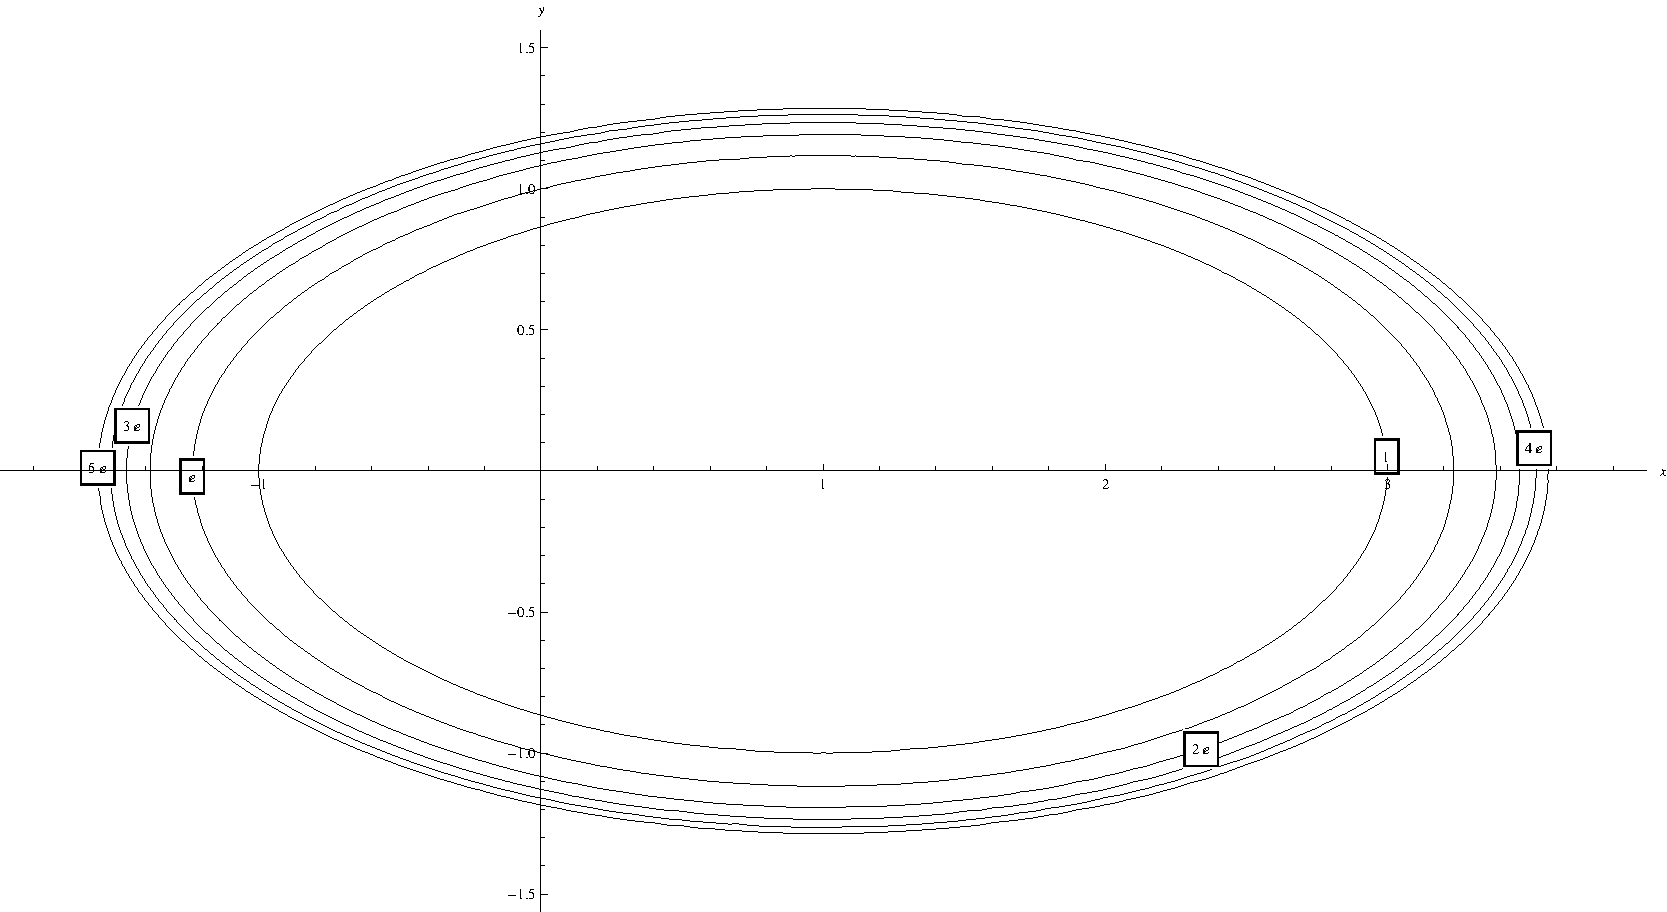
\includegraphics[width=\textwidth]{opg2_nivkurver.pdf} %trim=l b r t
	\caption{Niveaukurver}
	\label{fig:opg2_nivkurver}
	\end{center}
\end{figure}

Sk�ringer med $x$-aksen er 
\begin{align*}
	1 &= \dfrac{(x-1)^2}{5}\iff\\
	x &= \pm\sqrt{5}+1\implies\\
	x &\approx -1.24 \vee x \approx 3.24
\end{align*}
og sk�ringer med $y$-aksen er
\begin{align*}
	1 &= \dfrac{1}{5}+\dfrac{y^2}{\nicefrac{5}{4}}\iff\\
	y &= \pm 1
\end{align*}
Stor- og lilleaksernes l�ngde er
\begin{align*}
	a &= \sqrt{5} \approx 2,24\\
	b &= \sqrt{\frac{5}{4}} \approx 1,12
\end{align*}

P� figur \ref{fig:opg2_nivkurver} ses niveaukurver (hvor $K = 1, e, 2e, 3e, 4e, 5e$) afbilledet vha. \textit{Mathematica}
\section*{Opgave 3}\addcontentsline{toc}{section}{Opgave 3}\refstepcounter{section}
Det �nskes at finde volumen indesluttet af cylinderen
\begin{equation*}
	x^2+y^2=4
\end{equation*}
og afgr�nset af 
\begin{align*}
	z=x+y+4\\
	z=x-y\\
	z \geq 0
\end{align*}

\begin{figure}[htb]
	\begin{center}
	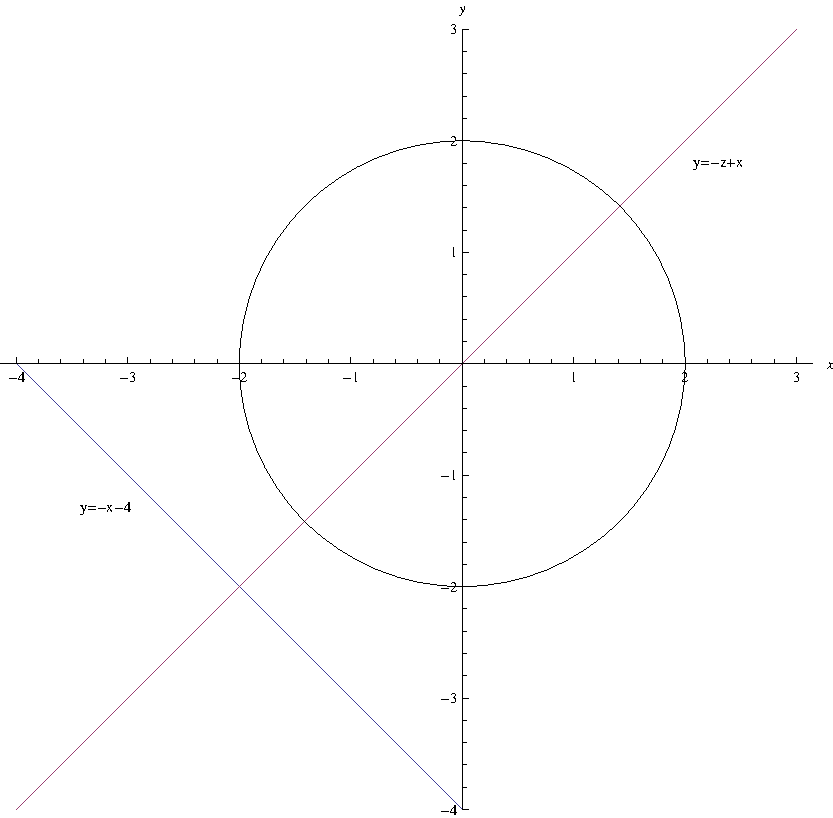
\includegraphics[width=0.7\textwidth]{opg3_z0} %trim=l b r t
	\caption{Problem afbilledet i $(x,y)$-planet hvor $z=0$}
	\label{fig:opg3_z0}
	\end{center}
\end{figure}

Cylinderen er symmetrisk om $z$-aksen (har centrum i $(0,0)$ i $(x,y)$-planet) og har radius $2$. For at f� en ide om, hvordan gr�nserne ser ud, ser vi p� $(x,y)$-planet i det $z=0$ (figur \ref{fig:opg3_z0})

P� figur \ref{fig:opg3_z0} ses det, at $z=x+y+4$ ikke ''sk�rer'' noget af cylinderen s� l�nge $z \geq 0$. Dog g�r $z=x-y$ lige igennem cylinderens midte n�r $z=0$, men fordi $z=x-y$ stiger eller falder lige meget p� begge sider af $z=0$ kan vi faktisk helt ignorere den afgr�nsning og bare bruge $z=0$. Det er ingen grund til f�rst at skulle finde den volume for s� at ''tr�kke den fra'' bagefter. Figur \ref{fig:opg3_x0} viser dette: Det skraverede omr�de er hvor $z=x-y$ er forskellig fra $z=0$ indenfor cylinderens sider.

\begin{figure}[htb]
	\begin{center}
	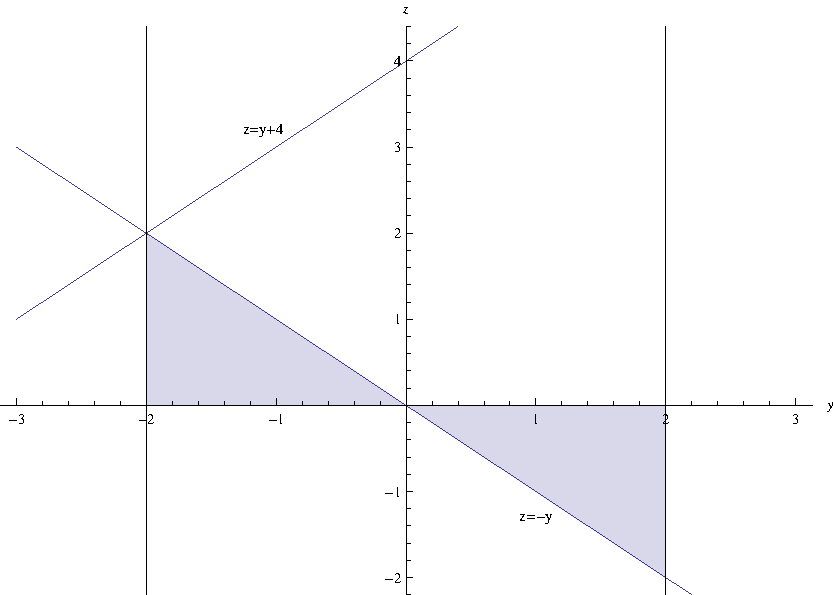
\includegraphics[width=0.84\textwidth]{opg3_x0} %trim=l b r t
	\caption{Problem afbilledet i $(z,y)$-planet hvor $x=0$. De lodrette streger er cylinderens sider.}
	\label{fig:opg3_x0}
	\end{center}
\end{figure}

Nu kan integralet s� opstilles. For at lette integrationen benyttes cylindriske koordinater. F�rst findes arealet af $r \, dz$, fra $z=0$ til vi rammer $z=x+y+4$. Radius skal summeres fra $0$ til $2$ og $\theta$ er en fuld cirkel fra $0$ til $2\pi$.
\begin{align*}
	\int_0^{2 \pi } \int_0^2 \int_0^{r \cos\theta +r \sin\theta +4} r \, dz \, dr \, d\theta 
\end{align*}

S�ledes kan vi evaluere integralet
\begin{align*}
	& \int_0^{2 \pi } \int_0^2 \int_0^{r \cos\theta +r \sin\theta +4} r \, dz \, dr \, d\theta \\
	&= \int_0^{2 \pi } \int_0^2 \left( r^2 \cos\theta + r^2 \sin\theta +4r \right) \, dr \, d\theta \\
	&= \int_0^{2 \pi } \left( \bigg[ \frac{1}{3}r^3 \cos\theta + \frac{1}{3}r^3 \sin\theta +2r^2 \bigg]_{0}^{2} \right) \, d\theta \\
	&= \int_0^{2 \pi } \left( \frac{8}{3} \cos\theta + \frac{8}{3} \sin\theta +8 \right) \, d\theta \\
	&= \bigg[ \frac{8}{3} \sin\theta - \frac{8}{3} \cos\theta +8\theta \bigg]_{0}^{2\pi} \\
	&= \left( -\frac{8}{3} + 16 \pi \right) - \left( -\frac{8}{3} \right) \\
	&= 16 \pi
\end{align*}
\section*{Opgave 4}\addcontentsline{toc}{section}{Opgave 4}\refstepcounter{section}
Vi har vektorfeltet
\[
	\mathbf{F} = 
	\begin{pmatrix}
		axy+3yz \\
		x^2+3xz+by^2z \\
		bxy+cy^3
	\end{pmatrix}
\]

hvor $a$, $b$ og $c$ er reelle konstanter. Det �nskes at bestemme integralet $I$
\[
	I = \int_{\mathcal{C}} \mathbf{F} \cdot d\mathbf{r}
\]
hvor $\mathcal{C}$ er en kurve fra $(0,1,-1)$ til $(2,1,1)$

\subsection*{a)}\addcontentsline{toc}{subsection}{a)}\refstepcounter{subsection}
Konstanterne $a$, $b$ og $c$ �nskes fundet, s�ledes at $I$ er uafh�ngig af kurvens vej. Vi ved, at hvis vektorfeltet $\mathbf{F}$ er konservativt, afh�nger $I$ netop \textit{ikke} af kurvens vej\footcite[866]{adamsessex}.

Hvis vektorfeltet $\mathbf{F}$ er konservativt eksisterer der en potentialefunktion $f$, s� $\mathbf{F} = \nabla f$. $I$ kan, idet vi kender $f$ ogs� skrives som\footcite[867]{adamsessex}
\[
	I = \int_{\mathcal{C}} \mathbf{F} \cdot d\mathbf{r} = \int_{\mathcal{C}} \nabla f \cdot d\mathbf{r} = f(P_1) - f(P_0)
\]
hvor kurven $\mathcal{C}$ g�r fra punktet $P_0$ til punktet $P_1$.

For at bestemme $f$ unders�ges ligheden $\mathbf{F} = \nabla f$
\begin{align*}
	\mathbf{F} &= \nabla f \implies \\
	F_1 \mathbf{i} + F_2 \mathbf{j} + F_3 \mathbf{k} &= \frac{\partial f}{\partial x} \mathbf{i} + \frac{\partial f}{\partial y} \mathbf{j} + \frac{\partial f}{\partial z} \mathbf{k}
\end{align*}

Hvert led kan s�ttes lig hinanden, s�
\[
	F_1 = \frac{\partial f}{\partial x}
\]
\[
	F_2 = \frac{\partial f}{\partial y}
\]
\[
	F_3 = \frac{\partial f}{\partial z}
\]

For at finde $f$ integreres den f�rste lighed med respekt til $x$ for at give et muligt udtryk for $f$. Derefter sammenlignes $f$, partielt differentieret mht. $y$ og $z$, for at opn� et mere fuldkomment udtryk for $f$. I l�bet af denne process kan konstanterne $a$, $b$ og $c$ samtidig bestemmes.
\begin{align*}
	\frac{\partial f}{\partial x} &= axy+3yz \implies\\
	f &= \int (axy+3yz) dx\\
	&= \frac{1}{2} ax^2y + 3xyz + g(y,z)
\end{align*}
Integrationskonstanten lader vi v�re en funktion $g$ af $y$ og $z$. Hvis $g(y,z)$ differentieres partielt mht. $x$ bliver den $0$ og ligheden g�lder.

Nu haves s�ledes et udtryk for $f$ som kan differentieres partielt mht. $y$
\begin{align*}
	\frac{\partial f}{\partial y} &= \frac{\partial}{\partial y} \left( \frac{1}{2} ax^2y + 3xyz + g(y,z) \right)\implies\\
	&= \frac{1}{2} ax^2 + 3xz + \frac{\partial g(y,z)}{\partial y}
\end{align*}

Dette udtryk sammenlignes med $F_2$ for at bestemme konstanter
\[
	x^2+3xz+by^2z = \frac{1}{2} ax^2 + 3xz + \frac{\partial \, g(y,z)}{\partial y}
\]

Vi ser at det m� betyde, at $a=2$ og 
\begin{align*}
	\frac{\partial \, g(y,z)}{\partial y} &= by^2z \implies\\
	g(y,z) &= \int (by^2z) dy\\
	&= \frac{1}{3}by^3z+h(z)
\end{align*}
Differentieres $g(y,z)$ mht. $y$ skal resultatet v�re 0, dvs. at $g$ h�jst kan v�re en funktion af $z$. Den kalder vi $h(z)$

Nu kan $g(y,z)$ inds�ttes i $f$
\[
	f = \frac{1}{2} ax^2y + 3xyz + \frac{1}{3}by^3z+h(z)
\]

Slutteligt differentieres $f$ partielt mht. $z$
\begin{align*}
	\frac{\partial f}{\partial z} &= \frac{\partial}{\partial z} \left( \frac{1}{2} ax^2y + 3xyz + \frac{1}{3}by^3z+h(z) \right)\\
	&= 3xy + \frac{1}{3}by^3 + \frac{\partial \, h(z)}{\partial z}
\end{align*}

og vi sammenligner med $F_3$
\[
	bxy+cy^3 = 3xy + \frac{1}{3}by^3 + \frac{\partial \, h(z)}{\partial z}
\]
hvor det ses, at $b=3$, $c=1$ og 
\begin{align*}
\frac{\partial \, h(z)}{\partial z} &= 0 \implies\\
h(z) &= k
\end{align*}
Differentieres en konstant $k$ bliver den $0$

Dermed kan et fuldkomment udtryk for potentialefunktionen $f$ opskrives idet konstanterne $h(z)$, $a$, $b$ og $c$ inds�ttes
\[
	f = x^2y + 3xyz + y^3z+k
\]

\subsection*{b)}\addcontentsline{toc}{subsection}{b)}\refstepcounter{subsection}
I denne opgave skal integralet $I$ bestemmes. I opgave 4a opstilledes f�lgende lighed 
\[
	I = \int_{\mathcal{C}} \mathbf{F} \cdot d\mathbf{r} = f(P_1) - f(P_0)
\]

Potentialefunktionen $f$ er allerede bestemt og v�rdierne for $a$, $b$ og $c$ er indsat, s� vi evaluerer blot udtrykket
\begin{align*}
	I &= f(2,1,1) - f(0,1,-1) \\
	&= (2^2 + 3(2) + 1) - (-1)\\
	&=12
\end{align*}
\newpage
\section*{Opgave 5}\addcontentsline{toc}{section}{Opgave 5}\refstepcounter{section}
Et vektorfelt er beskrevet ved
\[
	\mathbf{F} = 
	\begin{pmatrix}
		e^x - y^3 \\
		e^y + x^3 \\
		e^z
	\end{pmatrix}
\]

Denne opgave g�r ud p�, at beregne
\[
	\int_{\mathcal{C}} \mathbf{F} \cdot d\mathbf{r}
\]

hvor kurven $\mathcal{C}$ er givet ved
\[
	\mathbf{r}(t) = 
	\begin{pmatrix}
		\cos t \\
		\sin t \\
		\sin 2t
	\end{pmatrix}
\]
og $0 \leq t \leq 2\pi$

For at bestemme integralet vil vi benytte Stokes s�tning, som relaterer et linjeintegrale til et overfladeintegrale\footcite[913]{adamsessex}:
\[
	\oint_{\mathcal{C}} \mathbf{F} \cdot d\mathbf{r} = \iint_{\mathcal{S}} \mathrm{curl}\,\mathbf{F} \cdot \hat{\mathbf{N}} \, dS
\]

For at kunne bruge Stokes s�tning skal det vises, at kurven $\mathcal{C}$ ligger p� overfladen $z=2xy$. Det kan vi g�re ved at substituere de parametriske ligninger for kurven ind p� h�jresiden af ligningen for overfladen og anvende en trigonometrisk identitet
\begin{align*}
	z &= 2xy \implies \\
	z &= 2 \cos t \sin t\\
	&= \sin 2t
\end{align*}
Det ses, at alle punkter af kurven $\mathcal{C}$ tilfredsstiller ligningen for overfladen, s� kurven m� ligge p� overfladen.

For at evaluere integralet skal vi kende $\mathrm{curl}\,\mathbf{F}$
\[
	\mathrm{curl}\,\mathbf{F} = \mathbf{F} \times \nabla = \begin{vmatrix}
			\mathbf{i} & \mathbf{j} & \mathbf{k} \\
			\dfrac{\partial}{\partial x} & \dfrac{\partial}{\partial y} & \dfrac{\partial}{\partial z} \\
			e^x - y^3 &	e^y + x^3 &	e^z
		\end{vmatrix}
\]
\[
	= \left( \dfrac{\partial}{\partial y}(e^z) - \dfrac{\partial}{\partial z}(e^y + x^3) \right) \mathbf{i} +
		\left( \dfrac{\partial}{\partial z}(e^x - y^3) - \dfrac{\partial}{\partial x}(e^z) \right) \mathbf{j} +
		\left( \dfrac{\partial}{\partial x}(e^y + x^3) - \dfrac{\partial}{\partial y}(e^x - y^3) \right) \mathbf{k}
\]
\[
	= 3 \left( x^2 + y^2 \right) \mathbf{k}
\]

For en overflade med ligning $z=g(x,y)=2xy$ g�lder\footcite[885]{adamsessex}
\begin{align*}
	\hat{\mathbf{N}} \, dS &= \pm \left( -\dfrac{\partial g}{\partial x}\mathbf{i} -\dfrac{\partial g}{\partial y}\mathbf{j} + \mathbf{k} \right) dA \\
	&= (-2y\mathbf{i} - 2x\mathbf{j} + \mathbf{k}) \, dA
\end{align*}

Projektionen af kurven givet ved $\mathbf{r}(t)$ p� regionen $R$ i $xy$-planet er en enhedscirkel med centrum i $(0,0)$. Dvs
\begin{align*}
	\oint_{\mathcal{C}} \mathbf{F} \cdot d\mathbf{r} &= \iint_{\mathcal{S}} \mathrm{curl}\,\mathbf{F} \cdot \hat{\mathbf{N}} \, dS\\
	&= \iint_{R}3 \left( x^2 + y^2 \right)\mathbf{k} \cdot (-2y\mathbf{i} - 2x\mathbf{j} + \mathbf{k}) \, dA\\
	&= \iint_{R}3 \left( x^2 + y^2 \right) dA
\end{align*}

Med integralet og gr�nserne omskrevet til cylindriske koordinater bliver det let at evaluere integralet
\begin{align*}
	\oint_{\mathcal{C}} \mathbf{F} \cdot d\mathbf{r} &= \iint_{R}3 \left( x^2 + y^2 \right) dA\\
	&= \int_{0}^{2\pi} \int_{0}^{1} 3 r^2 \, r \, dr \, d\theta \\
	&= \dfrac{3 \pi}{2}
\end{align*}
\section*{Opgave 6}\addcontentsline{toc}{section}{Opgave 6}\refstepcounter{section}
Der skal findes en l�sning til den partielle differentialligning
\begin{equation*}
	3u_{xx}-12u_{xy}+9u_{yy}=0
\end{equation*}
hvor $u$ er en funktion af $x$ og $y$

Vi har at g�re med en 2. ordens partiel differentialligning p� formen $Au_{xx}+2Bu_{xy}+Cu_{yy}=F(x,y,u,u_x,u_y)$. Det ses at - fordi $AC-B^2<0$ - er ligningen hyperbolsk.

For at transformere differentialligningen til \textit{normal form} l�ses karakteristikligningen\footcite[551]{kreyzig}
\begin{align*}
	A\left(\frac{dy}{dx}\right)^2 - 2B\frac{dy}{dx} + C &= 0 \implies \\
	\frac{dy}{dx} &= \dfrac{B \pm \sqrt{B^2-AC}}{A} \implies \\
	\frac{dy}{dx} &= \dfrac{-6 \pm \sqrt{(-6)^2 - 3 \cdot 9}}{3} \implies \\
	\frac{dy}{dx} &= \left\{
	  \begin{array}{l}
	   -3 \\
	   -1 \\
	  \end{array} \right. \implies \\
	y &= \left\{
	  \begin{array}{l}
	   -3x+K \\
	   -1x+K \\
	  \end{array} \right.
\end{align*}

L�sningerne til karakteristikligningen lader vi v�re
\begin{align*}
	v(x,y) &= 3x+y \\
	w(x,y) &= x+y 
\end{align*}
s�
\begin{align*}
	\frac{\partial v}{\partial x} &= 3\\
	\frac{\partial v}{\partial y} &= 1\\
	\frac{\partial w}{\partial x} &= 1\\
	\frac{\partial w}{\partial y} &= 1
\end{align*}

Ved brug af k�dereglen f�s
\begin{align*}
	\frac{\partial u}{\partial x} &= \frac{\partial u}{\partial v} \frac{\partial v}{\partial x} + \frac{\partial u}{\partial w} \frac{\partial w}{\partial x} = 3 \frac{\partial u}{\partial v} + \frac{\partial u}{\partial w} \\
	\frac{\partial u}{\partial y} &= \frac{\partial u}{\partial v} \frac{\partial v}{\partial y} + \frac{\partial u}{\partial w}\frac{\partial w}{\partial y} = \frac{\partial u}{\partial v} + \frac{\partial u}{\partial w}
\end{align*}

Vi ser nu p� den oprindelige differentialligning $3u_{xx}-12u_{xy}+9u_{yy}$ for, ledvist, at bestemme de dobbeltdifferentierede - igen ved brug af k�dereglen (den virker ogs� p� et differentieret led idet det selv er en funktion af $x$ og $y$)
\begin{align*}
		u_{xx} &= \frac{\partial}{\partial x} \frac{\partial u}{\partial x} = \frac{\partial }{\partial x} \left( 3 \frac{\partial u}{\partial v} + \frac{\partial u}{\partial w} \right)\\
		&= 3 \left( \left( \frac{\partial }{\partial v} \frac{\partial u}{\partial v} \right) \frac{\partial v}{\partial x} + \left( \frac{\partial }{\partial w} \frac{\partial u}{\partial v} \right) \frac{\partial w}{\partial x} \right) +
			\left( \frac{\partial }{\partial v} \frac{\partial u}{\partial w} \right) \frac{\partial v}{\partial x} + \left( \frac{\partial }{\partial w} \frac{\partial u}{\partial w} \right) \frac{\partial w}{\partial x}\\
		&= 9 \frac{\partial^2 u}{\partial v^2} + 6 \frac{\partial^2 u}{\partial v \partial w} + \frac{\partial^2 u}{\partial w^2}
	\\
%--
	u_{xy} &=	\frac{\partial}{\partial y}\frac{\partial u}{\partial x} = \frac{\partial }{\partial y} \left( 3 \frac{\partial u}{\partial v} + \frac{\partial u}{\partial w} \right)\\
	&= 3 \left( \left( \frac{\partial }{\partial v} \frac{\partial u}{\partial v} \right) \frac{\partial v}{\partial y} + \left( \frac{\partial }{\partial w} \frac{\partial u}{\partial v} \right) \frac{\partial w}{\partial y} \right) +
			\left( \frac{\partial }{\partial v} \frac{\partial u}{\partial w} \right) \frac{\partial v}{\partial y} + \left( \frac{\partial }{\partial w} \frac{\partial u}{\partial w} \right) \frac{\partial w}{\partial y}\\
		&= 3 \frac{\partial^2 u}{\partial v^2} + 4 \frac{\partial^2 u}{\partial v \partial w} + \frac{\partial^2 u}{\partial w^2}
	\\
%--
	u_{yy} &=	\frac{\partial}{\partial y}\frac{\partial u}{\partial y} = \frac{\partial}{\partial y} \left( \frac{\partial u}{\partial v} + \frac{\partial u}{\partial w} \right)\\
	&= \left( \frac{\partial }{\partial v} \frac{\partial u}{\partial v} \right) \frac{\partial v}{\partial y} + \left( \frac{\partial }{\partial w} \frac{\partial u}{\partial v} \right) \frac{\partial w}{\partial y} +
			\left( \frac{\partial }{\partial v} \frac{\partial u}{\partial w} \right) \frac{\partial v}{\partial y} + \left( \frac{\partial }{\partial w} \frac{\partial u}{\partial w} \right) \frac{\partial w}{\partial y}\\
	&= \frac{\partial^2 u}{\partial v^2} + 2 \frac{\partial^2 u}{\partial v \partial w} + \frac{\partial^2 u}{\partial w^2}
\end{align*}

Indsat i differentialligningen f�s
\begin{align*}
	3u_{xx}-12u_{xy}+9u_{yy} = 0& \\ \implies &\\
	3 \left( 9 \frac{\partial^2 u}{\partial v^2} + 6 \frac{\partial^2 u}{\partial v \partial w} + \frac{\partial^2 u}{\partial w^2} \right)
	- 12 \left( 3 \frac{\partial^2 u}{\partial v^2} + 4 \frac{\partial^2 u}{\partial v \partial w} + \frac{\partial^2 u}{\partial w^2} \right)
	+ 9 \left( \frac{\partial^2 u}{\partial v^2} + 2 \frac{\partial^2 u}{\partial v \partial w} + \frac{\partial^2 u}{\partial w^2} \right) = 0&\\
	\implies &\\
	-12 \frac{\partial^2 u}{\partial v \partial w} = 0& 
\end{align*}

Det fort�ller os, at $\dfrac{\partial u}{\partial w}$ differentieret mht. $v$ er 0 og s�ledes m� $\dfrac{\partial u}{\partial w}$ v�re en funktion kun afh�ngig af $w$ - lad os kalde den $f$: 
\[
	\frac{\partial u}{\partial w}=f(w)
\]
Integreres en gang mht. $w$ f�s
\begin{align*}
	u(v,w) &= \int f(w) \, dw \\
	&= F(w) + G(v)
\end{align*}
hvor integrationskonstanten er $G(v)$ - siden vi kun integrerer mht. $w$ kan den stadig godt v�re en funktion af $v$.
Det er den generelle l�sning p� ligningen. Som funktion af $x$ og $y$ bliver l�sningen
\[
	u(x,y) = F(x+y) + G(3x+y)
\]
%V�lger vi f. eks. $F(x)= x^2$ og $G(x)= \sin x$ kan vi tjekke om l�sningen er ok
%\begin{align*}
%	u(x,y) = (x+y)^2 + \sin(3x+y)\\
%\end{align*}
\section*{Opgave 7}\addcontentsline{toc}{section}{Opgave 7}\refstepcounter{section}
F�lgende differentialligning �nskes l�st
\[
	u_{tt}+au_t=c^2u_{xx} ,\quad 0\leq x \leq 1 ,\quad t \geq 0
\]
hvor $u$ er en funktion af $x$ og $t$: $u(x,t)$. $a$ og $c$ er konstanter.

Randbetingelser for ligningen er
\begin{align*}
	u(0,t) &= 0\\
	u(L,t) &= 0
\end{align*}
og begyndelsesbetingelserne er
\begin{align*}
	u(x,0) &= 0\\
	u_t(x,0) &= g(x)
\end{align*}

%%%%%%%%%%%
\subsection*{a)}\addcontentsline{toc}{subsection}{a)}\refstepcounter{subsection}
F�rste trin af l�sningen er at omskrive den partielle differentialligning til to ODE'er ved brug af metoden ''seperation af variable''. Det antages at $u(x,t)=F(x)\,G(t)$

F�rst differentieres $u(x,t)=F(x)\,G(t)$ for at opn� de led, der beh�ves i den oprindeligt givne differentialligning. Prikkerne over $G$ angiver, at den er differentieret mht. $t$ (tid)
\begin{align*}
	u(x,t) &= F(x)\,G(t) \implies \\
	u_{xx} &= F'' G \\
	u_{tt} &= F \ddot{G} \\
	u_{t} &= F \dot{G}
\end{align*}

Inds�ttes disse i den oprindelige differentialligning f�s
\[
	F \ddot{G} + a F \dot{G} = c^2 F'' G
\]

Ligningen arrangeres s� $F$- og $G$-leddene kommer til at st� p� hver sin side af lighedstegnet
\begin{align*}
	F \ddot{G} + a F \dot{G} &= c^2 F'' G \iff \\
	\frac{\ddot{G}}{G} + a \frac{\dot{G}}{G} &= c^2 \frac{F''}{F}
\end{align*}

Nu er venstresiden kun afh�ngig af $t$ og h�jresiden kun af $x$. Det vil sige, at begge sider m� v�re konstante - �ndres kun enten $x$ eller $t$ ville ligheden ikke g�lde, hvis begge sider ikke var konstante. Alts� har vi
\[
	\frac{\ddot{G}}{G} + a \frac{\dot{G}}{G} = c^2 \frac{F''}{F} = k
\]
hvor $k$ kaldes seperationskonstanten. Den er endnu arbitr�r.

Nu kan vi inddele i to ordin�re differentialligninger
\begin{align*}
	\frac{\ddot{G}}{G} + a \frac{\dot{G}}{G} = c^2 \frac{F''}{F} &= k \implies \\
	c^2 F'' - k F &= 0 \\
	\ddot{G} + a \dot{G} - k G &= 0
\end{align*}

%%%%%%%%%%%
\subsection*{b)}\addcontentsline{toc}{subsection}{b)}\refstepcounter{subsection}
Vi skal nu bestemme l�sninger til $F(x)$ og $G(t)$ s� de opfylder randbetingelserne. Dvs f�lgende skal g�lde for alle $t$
\begin{align*}
	u(0,t) &= F(0)\,G(t) = 0\\
	u(L,t) &= F(L)\,G(t) = 0
\end{align*}

Vi viser, at seperationskonstanten, $k$ m� v�re negativ: Hvis $k=0$ f�r vi
\[
	c^2 F''= 0
\]

hvis karakterligning har roden $r=\nicefrac{0}{2c^2}=0$. En l�sning er $F=e^{rx}=1$. Alts� bliver $F''=0$ og den har den generelle l�sning $F=ax+b$ og fordi $u(0,t) = F(0)$ og $G(t) = 0$ bliver $a=b=0$ s� $F=0$ hvilket g�r at den oprindelige ligning bliver $u(x,y)=F(x)\,G(t)=0$ hvilket ikke er s�rlig interessant for os.

For en positiv $k=v^2$ har vi
\[
	c^2 F'' - v^2 F = 0
\]
hvis karakterligning har r�dderne $r_1=\nicefrac{v}{c}$ og $r_2=-\nicefrac{v}{c}$ og dermed l�sningen
\[
	F(x) = Ae^{\frac{v}{c} x}+Be^{-\frac{v}{c} x}
\]
s�
\[
	F(0) = F(L) = A+B = Ae^{\frac{v}{c} L}+Be^{-\frac{v}{c} L} = 0
\]

Heraf kan vi se, at $F=A=B=0$ som f�r. Denne l�sning er alts� heller ikke interessant.

Til sidst ser vi p� l�sningen for $F$ n�r $k$ er valgt negativ: $k = -u^2$. Da f�r vi 
\[
	c^2 F'' + u^2 F = 0
\]

hvis karakterligning har r�dderne $r=\pm \, \mathrm{i} \, \dfrac{u}{c}$ og s�ledes l�sningen
\[
	F(x) = A \cos\left(\frac{u}{c} x\right) + B \sin\left(\frac{u}{c} x\right)
\]

og $F(0)$ bliver 
\begin{align*}
	F(0) = A \cos\left(\frac{u}{c} \cdot 0\right) + B \sin\left(\frac{u}{c} \cdot 0\right) &=0 \implies \\
	A &= 0
\end{align*}

da $A=0$ bliver $F(L)$
\[
	F(L) = 0 = B \sin\left( \frac{u}{c} L \right)
\]

Vi m� v�lge $B \neq 0$ da vi eller f�r $F=0$ som f�r. Dvs at $\sin\left(\dfrac{u}{c} L\right) = 0$ f�r $F(L) = 0$ er opfyldt. Alts� m�
\[
	\frac{u L}{c} = n \pi \iff \frac{u}{c} = \frac{n \pi}{L},\quad (n=\dots, -1, 0, 1, 2, \dots)
\]

S�ttes f. eks. $B=1$ opn�s uendelig mange l�sninger: $F(x)=F_n(x)$ hvor
\[
	F_n(x) = \sin \left( \frac{n \pi}{L} x \right) ,\quad (n=1, 2, 3, \dots)
\]

%%%%%%%%%%%
\subsection*{c)}\addcontentsline{toc}{subsection}{c)}\refstepcounter{subsection}
Nu kan vi ogs� l�se $\ddot{G} + a \dot{G} - k G = 0$ hvor $k = -u^2 = -\left(\dfrac{n \pi c}{L}\right)^2$
\begin{align*}
	\ddot{G} + a \dot{G} + \left(\frac{n \pi c}{L}\right)^2 G &= 0 \implies \\
	\ddot{G} + a \dot{G} + \lambda_n^2 G &= 0
\end{align*}

hvor
\[
	\lambda_n = \frac{n \pi c}{L}
\]

Der l�ses, idet $a = 2 \lambda$, hvorved kompliment�rligningen bliver
\[
	r^2+2 \lambda r + \lambda^2 =0
\]

Diskriminanten til kompliment�rligningen er da 
\[
	D=(2 \lambda)^2 - 4 \lambda^2 =0
\]

De to ens r�dder til kompliment�rligningen er
\[
	r=\frac{-2 \lambda}{2}= - \lambda
\]

og den generelle l�sning af $G$ bliver 
\[
	G(t) = A e^{- \lambda t} + B t e^{- \lambda t}
\]

Dermed f�s
\begin{align*}
	u(x,t) &= F(x)\,G(t) \implies \\
	u(x,t) &= \sin \left( \frac{n \pi x}{L} \right) \left(A e^{- \lambda t} + B t e^{- \lambda t} \right)
\end{align*}

Vi ser p� begyndelsesbetingelserne hvor
\begin{align*}
		u(x,0) = \sin \left( \frac{n \pi x}{L} \right) \left(A  \right) &= 0 \implies \\
		A &= 0
\end{align*}

og s�
\begin{align*}
	u(x,t) &= B t e^{- \lambda t} \sin \left( \frac{n \pi x}{L} \right)
\end{align*}





%% Appendiks
\clearpage
\appendix


%%% Litteraturliste
\section{Referencer}
%\nocite{*} % Inkluderer alle poster i bibl.bib-filen (dvs. kun skriv litteratur ind vi rent faktisk har brugt)
\printbibliography[heading=bibempty]







\end{document}